\chapter*{Введение}\label{chap:overview}
\addcontentsline{toc}{chapter}{Введение} % This is a hack

\section{Компьютерная симуляция}

Использование компьютерного моделирования в процессе проектирования позволяет заметно сократить  среднее время, проходящее от момента предложения концепции новой системы до поступления на рынок первых образцов готовой продукции. Это происходит благодаря т. н. «сдвигу влево» (\textit{англ.} shift left) всей существующей методологии, что позволяет совмещать многие процессы параллельно во времени, так как часть из них может быть начата гораздо раньше, чем это было возможно ранее, и эффективно сокращать цикл разработки (рис.~\ref{fig:shift-left}).

\begin{figure}[htb]
    \centering
    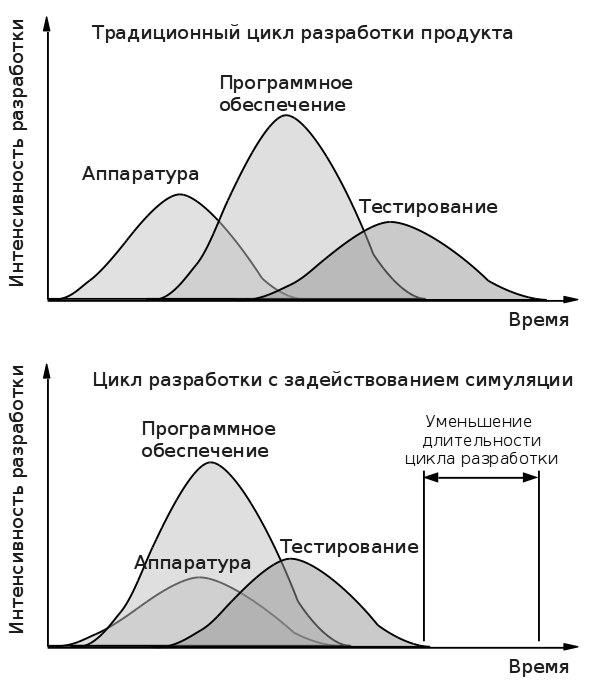
\includegraphics[width=0.6\textwidth]{./shift-left}
    \caption[Сдвиг влево]{Сдвиг влево --- возможность совместить моменты начала отдельных стадий проектирования новых цифровых систем, таким образом сокращая цикл разработки и уменьшая время вывода их на рынок}
    \label{fig:shift-left}
\end{figure}

Программное обеспечение для имитационного моделирования используется для тестирования и исследования производительности, функциональных и иных свойств вычислительных систем на стадиях их раннего проектирования, когда реальные образцы соответствующей аппаратуры ещё недоступны. Кроме того, оно позволяет писать приложения для таких систем заранее.

Задача данного цикла лабораторных работ --- познакомить слушателей с новейшими достижениями в области компьютерной симуляции, связанными с эффективным созданием моделей, максимально точно представляющих аппаратные средства и при этом имеющих приемлемую скорость работы, получаемую благодаря эффективному задействованию имеющихся вычислительных ресурсов. Изучение проводится на программном продукте Wind River\textregistered\ Simics (в дальнейшем просто Simics), который в настоящее время является одним из самых современных инструментов разработки, тестирования и исследования цифровых компьютерных систем и используется как в промышленности, так и в научной среде. Несмотря на это, почти все рассматриваемые вопросы включают в себя идеи и концепции, общие для разных симуляторов.

\section{Предварительные замечания}

Для максимально эффективного усвоения материала данного пособия читателю рекомендуется иметь начальные знания по архитектуре ЭВМ. Желательно понимание общих принципов работы операционных систем, а также знакомство как  минимум с одним языком программирования.

\section{Обозначения}
При первом использовании терминов, заимствованных из английского языка и не имеющих известных авторам общепринятых переводов на русский язык, в скобках после них будут указываться оригинальные термины.

Всюду в тексте данной работы будут использованы следующие шрифтовые выделения и обозначения.

\begin{itemize*}
    \item Обычный текст используется для основного материала.
    \item \texttt{Моноширинный текст} вводится для исходных текстов программ на различных (псевдо) языках программирования и их ключевых слов,  имён регистров устройств, листингов машинного кода.
    \item \textit{Наклонный текст} используется для выделения новых понятий.
    \item \textbf{Полужирный текст} используется для обозначения элементов графического интерфейса: имён окон, пунктов меню и т.п.
    \item Числа в шестнадцатеричной системе счисления имеют префикс \textbf{0x} (например, 0x12345abcd), в двоичной системе счисления --- суффикс \textbf{b} (например, 10010011b).
    \item Команды, которые необходимо вводить в строку приглашения Simics, имеют префикс \texttt{simics>}:
    \begin{lstlisting}
simics> list-objects
    \end{lstlisting}
    \item Команды, которые необходимо вводить в строку приглашения командной строки Bash, имеют префикс \texttt{\$} для обычного пользователя или \texttt{\#} для команд, выполняемых суперпользователем root:
    \begin{lstlisting}
$ ./simics targets/x86-x58-ich10/viper.simics
# mount /dev/sdb /mnt/disk
    \end{lstlisting}

    \item Обязательные аргументы команд указаны в угловых скобках, необязательные --- в квадратных, например:
    \begin{lstlisting}
$ command <mandatory argument> [optional argument]
    \end{lstlisting}

\end{itemize*}

